\chapter{De los modos de momento a los campos cuánticos locales}

¿Qué es un campo cuántico y cómo se relaciona con las partículas? La herramienta matemática básica es el oscilador armónico. Un campo contiene muchos modos de oscilación posibles; cuantizar el campo equivale a reunir un oscilador armónico cuántico por cada modo. La construcción se aprecia con mayor facilidad primero en un espacio periódico finito, donde los modos permitidos forman una lista discreta.

\section{Espacio periódico y números de onda permitidos}

Tomemos una coordenada espacial \(x\) e identifiquemos los puntos separados por una distancia \(L\). Podemos imaginar el espacio como un círculo de circunferencia \(L\). Este es un recurso útil para trabajar en un volumen finito. En un intervalo finito con extremos, una onda viajera se refleja en ellos. En un intervalo periódico, puede continuar en cualquiera de las dos direcciones sin reflejarse. Se conserva la simetría de traslación y, por tanto, el momento, mientras se dejan temporalmente de lado las complicaciones del volumen infinito.

Una onda plana tiene la forma
\begin{equation}
e^{ikx}.
\end{equation}
Después de dar una vuelta al círculo, debe recuperar su valor original. Como la onda vale \(1\) en \(x=0\), la periodicidad exige
\begin{equation}
e^{ikL}=1.
\end{equation}
¿Por qué un múltiplo entero de \(2\pi\) satisface esta condición? La fórmula de Euler da
\begin{align}
e^{i2\pi n}
&=\cos(2\pi n)+i\sin(2\pi n)\\
&=1,
\qquad n\in\mathbb Z.
\end{align}
El coseno vale \(1\) y el seno \(0\) después de cualquier número entero de ciclos. Por consiguiente,
\begin{equation}
kL=2\pi n,
\qquad
k=\frac{2\pi n}{L},
\qquad n\in\mathbb Z.
\end{equation}
La cantidad \(k\) es el número de onda. El entero \(n\) identifica un número de onda permitido; todavía no cuenta partículas.

La misma condición puede expresarse en términos de la longitud de onda. Una longitud de onda es la distancia en la que la fase avanza un ciclo completo, de modo que
\begin{equation}
k\lambda=2\pi,
\qquad
k=\frac{2\pi}{\lambda}.
\end{equation}
Una longitud de onda grande corresponde a un número de onda pequeño, y una longitud de onda pequeña, a uno grande. La condición de periodicidad indica que alrededor del círculo cabe un número entero de longitudes de onda.

Para una onda cuántica, el momento es
\begin{equation}
p=\frac{h}{\lambda}
=\frac{2\pi\hbar}{\lambda}
=\hbar k.
\end{equation}
Así, \(k\) y \(p\) solo difieren en el factor \(\hbar\). Los valores positivos y negativos de \(k\) describen ondas que se mueven en direcciones opuestas y partículas con momento dirigido en sentidos opuestos. En unidades en las que \(\hbar=1\), es habitual llamar momento a \(k\) sin hacer más distinciones.

Para cada \(k\) permitido, puede haber cierto número de cuantos en ese modo. Esto introduce un segundo entero:
\begin{equation}
n(k)=\text{number of quanta with wave number }k.
\end{equation}
Se denomina número de ocupación. El entero de \(k=2\pi n/L\) identifica el modo; \(n(k)\) indica cuántas partículas ocupan ese modo. Hay que especificar los números de ocupación tanto para los valores negativos como para los positivos de \(k\).

\begin{classroomqa}
\lecturetimestamp{00:11:58}
\audiencequestion{¿Es \(k\) en sí mismo un entero?}
\lecturerresponse{No. El número de onda es un múltiplo entero de \(2\pi/L\): \(k=2\pi n/L\). El entero \(n\) de esa fórmula identifica el momento permitido y es distinto del número de ocupación \(n(k)\), que cuenta los cuantos del modo.}
\end{classroomqa}

\section{Estados de número de ocupación y operadores de modo}

Un estado cuántico es un vector, o elemento lineal. Los vectores de estado se pueden sumar y multiplicar por números, y los operadores actúan sobre ellos para producir otros vectores de estado. Las magnitudes reales observables se representan mediante operadores hermíticos. Estos hechos elementales son pertinentes aquí porque tanto el estado de muchas partículas como el campo se construirán mediante combinaciones lineales y operadores.

Sea
\begin{equation}
k_j=\frac{2\pi j}{L},
\qquad j\in\mathbb Z.
\end{equation}
Una forma práctica de identificar un estado de muchas partículas consiste en usar la secuencia completa de números de ocupación. Con la abreviatura \(n_j\equiv n(k_j)\) para los elementos que aparecen en la expresión, escribimos
\begin{equation}
\big|\{n(k_j)\}\big\rangle
=
\big|\ldots,n_{-2},n_{-1},n_0,n_1,n_2,\ldots\big\rangle.
\end{equation}
El elemento \(n(k_1)\) es el número de partículas en el primer modo de momento positivo; \(n(k_2)\) es el número en el segundo, y así sucesivamente. La secuencia se extiende indefinidamente en ambas direcciones.

\begin{figure}[t]
\centering
\includegraphics[width=0.72\textwidth]{lecture_03_figure_02.png}
\caption{Número de ocupación \(n(k)\) para un modo de momento permitido.}
\lectureframe{00:15:04}
\end{figure}

Cada modo de momento es un oscilador armónico. Por tanto, tiene un operador de subida y uno de bajada. La notación que al principio se escribió como \(a^{+}(k)\) y \(a^{-}(k)\) se escribirá como \(a^\dagger(k)\) y \(a(k)\). Actúan así:
\begin{align}
a^\dagger(k)\big|\ldots,n(k),\ldots\big\rangle
&=
\sqrt{n(k)+1}\notag\\
&\quad{}\times
\big|\ldots,n(k)+1,\ldots\big\rangle,
\\
a(k)\big|\ldots,n(k),\ldots\big\rangle
&=
\sqrt{n(k)}\,
\big|\ldots,n(k)-1,\ldots\big\rangle.
\end{align}
El operador \(a^\dagger(k)\) va a la posición correspondiente a \(k\), aumenta esa ocupación en una unidad y multiplica el estado por \(\sqrt{n(k)+1}\). El operador \(a(k)\) reduce la ocupación de esa misma posición y aporta el factor \(\sqrt{n(k)}\). Hay un par de estos operadores por cada momento permitido.

\begin{figure}[t]
\centering
\includegraphics[width=0.58\textwidth]{lecture_03_figure_03.png}
\caption{Operadores de creación y aniquilación asociados al modo de momento \(k\).}
\lectureframe{00:17:14}
\end{figure}

\section{Los coeficientes de Fourier se convierten en operadores}

La conexión entre estos operadores del oscilador y un campo parte de una serie de Fourier clásica ordinaria. Un campo clásico complejo en el intervalo periódico se puede escribir como
\begin{align}
\psi(x)&=\sum_k \alpha(k)e^{ikx},\\
\psi^*(x)&=\sum_k \alpha^*(k)e^{-ikx},
\end{align}
donde cada suma recorre los valores permitidos de \(k=2\pi n/L\). Esto equivale a desarrollar el campo en senos y cosenos.

El campo complejo tiene una parte real y otra imaginaria. Su conjugado complejo cambia el signo de la parte imaginaria, y \(e^{ikx}\) se convierte en \(e^{-ikx}\). Especificar todos los coeficientes \(\alpha(k)\) determina el campo clásico. Una vez conocido \(\alpha(k)\), no hace falta especificar \(\alpha^*(k)\) por separado, pero las partes real e imaginaria de cada coeficiente son magnitudes reales independientes. Se pueden medir como las amplitudes de las componentes de Fourier correspondientes. En este sentido, un coeficiente complejo reúne dos observables clásicos.

La cuantización sustituye estos coeficientes clásicos de Fourier por operadores. Como una igualdad ordinaria identificaría objetos de distinta naturaleza, es preferible escribir una regla de sustitución:
\begin{equation}
\alpha(k)\rightsquigarrow a(k),
\qquad
\alpha^*(k)\rightsquigarrow a^\dagger(k).
\end{equation}
Con una elección coherente de los signos de Fourier, los campos cuánticos se definen así:
\begin{align}
\Psi(x)&=\sum_k a(k)e^{ikx},\\
\Psi^\dagger(x)&=\sum_k a^\dagger(k)e^{-ikx}.
\end{align}
\editorialnote{La exposición oral cambia y más adelante pone en duda la convención de signos de Fourier. El par conjugado que se usa aquí sigue la convención que aparece en la expansión del campo más clara y en el cálculo con estados de posición: \(\Psi\) lleva \(e^{ikx}\) y \(\Psi^\dagger\) lleva \(e^{-ikx}\). Invertir todos los signos de forma coherente describiría la misma construcción.}

Por ahora, esto es una definición: un campo cuántico es una suma de Fourier cuyos coeficientes son operadores. Una justificación más completa tendría que mostrar cómo estos operadores reproducen los coeficientes clásicos en un límite adecuado, lo que requiere cierta dinámica. Dejaremos esa cuestión para más adelante. Lo que ya está claro es que el campo mismo es un operador y que las relaciones entre sus coeficientes de Fourier son las relaciones de creación y aniquilación de los osciladores armónicos.

\begin{classroomqa}
\lecturetimestamp{00:26:48}
\audiencequestion{¿Introducir operadores de creación y aniquilación significa que la dinámica necesariamente crea y destruye partículas?}
\lecturerresponse{No. Los operadores son operaciones matemáticas que cambian los números de ocupación. Que las leyes de la naturaleza cambien o no el número de partículas es una cuestión dinámica. Si la dinámica permite esos cambios, estos operadores ofrecen el lenguaje natural para describirlos.}
\end{classroomqa}

\section{Dispersión y número variable de partículas}

Consideremos primero un proceso que no cambia el número de partículas. Supongamos que la única partícula presente inicialmente tiene momento \(k_7\). En la notación de números de ocupación, su estado tiene un \(1\) en la séptima posición y ceros en todas las demás:
\begin{equation}
|k_7\rangle
=
|\ldots,0,\underset{k_7}{1},0,\ldots\rangle.
\end{equation}
Un proceso de dispersión cambia su momento de \(k_7\) a \(k_9\). El operador que efectúa exactamente este cambio es
\begin{equation}
a^\dagger(k_9)a(k_7).
\end{equation}
El operador situado más a la derecha actúa primero: elimina la partícula de la posición \(k_7\). Luego, el operador de la izquierda crea una partícula en la posición \(k_9\).

\begin{classroomqa}
\lecturetimestamp{00:31:37}
\audiencequestion{¿Cómo intervienen los factores de raíz cuadrada en este proceso \(k_7\to k_9\)?}
\lecturerresponse{El factor de aniquilación es \(\sqrt{n(k_7)}=\sqrt{1}=1\). Tras esa eliminación, el sistema queda en el estado con todas las ocupaciones nulas. Como el modo \(k_9\) está vacío, el factor de creación es \(\sqrt{n(k_9)+1}=\sqrt{1}=1\). Por tanto, en este ejemplo de una partícula, ninguno de los dos factores cambia el coeficiente numérico.}
\end{classroomqa}

Llevemos a cabo ambos pasos. La aniquilación da
\begin{align}
a(k_7)|k_7\rangle
&=
\sqrt{1}\,|\ldots,0,0,0,\ldots\rangle\\
&=|0\rangle.
\end{align}
El estado con todas las ocupaciones nulas es el vacío. Es el estado sin partículas y, en este conjunto sencillo de osciladores, también es el estado fundamental. La creación en el modo \(k_9\), que está vacío, da entonces
\begin{equation}
a^\dagger(k_9)|0\rangle
=\sqrt{0+1}\,|k_9\rangle
=|k_9\rangle.
\end{equation}
Por consiguiente,
\begin{equation}
a^\dagger(k_9)a(k_7)|k_7\rangle=|k_9\rangle.
\end{equation}
En términos de las ocupaciones de cada posición, la única partícula \(1\) simplemente ha pasado del séptimo modo de momento al noveno. Como ninguna ocupación llegó a superar la unidad, ambos factores de raíz cuadrada valieron uno. Estos factores serán importantes en cuanto intervenga un modo que ya esté ocupado.

Este proceso de una partícula a otra también se podría describir mediante la mecánica cuántica ordinaria de una sola partícula: una partícula cambia de momento. El lenguaje de los números de ocupación se vuelve indispensable cuando puede cambiar el número de partículas. Por ejemplo,
\begin{equation}
a^\dagger(k_9)a^\dagger(k_{16})a(k_7)|k_7\rangle
=|k_9,k_{16}\rangle
\end{equation}
describe el cambio matemático de una partícula incidente en el modo \(k_7\) a dos partículas salientes, una en \(k_9\) y otra en \(k_{16}\). Un blanco puede absorber la partícula incidente, emitir las dos partículas salientes y adquirir el retroceso necesario. Un proceso así no se puede representar en un espacio de Hilbert restringido a una partícula, pero encaja de manera natural en un espacio de estados cuyas ocupaciones pueden variar. La expresión con operadores no es por sí sola una ley de la naturaleza: es el lenguaje en el que se puede escribir una ley que cambie el número de partículas.

\section{Un operador de campo en un punto}

¿Qué crea el operador en el espacio de posiciones \(\Psi^\dagger(x)\)? Los estados cuánticos forman un espacio lineal: se pueden sumar estados de momento con coeficientes complejos para formar un estado nuevo. Partamos del vacío. Como todos los modos están vacíos,
\begin{equation}
\Psi(x)|0\rangle=0.
\end{equation}
El cero de la derecha es el vector nulo: un operador de aniquilación no puede encontrar ninguna partícula que eliminar.

El campo conjugado actúa de otra manera:
\begin{align}
\Psi^\dagger(x)|0\rangle
&=\sum_k e^{-ikx}a^\dagger(k)|0\rangle\\
&=\sum_k e^{-ikx}|k\rangle,
\end{align}
donde
\begin{equation}
|k\rangle=a^\dagger(k)|0\rangle
\end{equation}
es el estado de una partícula con momento \(\hbar k\).

\begin{figure}[t]
\centering
\includegraphics[width=0.70\textwidth]{lecture_03_figure_05.png}
\caption{El estado formal en el espacio de posiciones \(\Psi^\dagger(x)|0\rangle\) desarrollado en estados de momento de una partícula.}
\lectureframe{00:43:16}
\end{figure}

Formalmente, y salvo un factor de normalización, la suma es el estado generalizado de posición de la mecánica cuántica de una partícula.\footnote{Con infinitos modos de momento, un estado de posición exactamente localizado no es normalizable. Si se impone un corte finito en el momento y se normaliza la suma truncada, se obtiene un paquete de ondas muy localizado, centrado en \(x\).}Los estados propios del momento, combinados con los coeficientes \(e^{-ikx}\), producen localización en \(x\). En este sentido formal,
\begin{equation}
\Psi^\dagger(x)\ \text{creates a particle at position }x,
\end{equation}
mientras que
\begin{equation}
\Psi(x)\ \text{annihilates a particle at position }x.
\end{equation}
El operador de modo \(a^\dagger(k)\) crea una partícula con momento definido. El operador de campo \(\Psi^\dagger(x)\) crea la superposición coherente de los estados de momento permitidos, formalmente localizada en \(x\).

En la suma formal sin normalizar, cada coeficiente \(e^{-ikx}\) tiene módulo uno. Con un corte finito, el estado truncado y normalizado tiene coeficientes de igual módulo para los momentos que se conservan, mientras que sus fases producen un paquete de ondas muy localizado cerca de \(x\). Esta es la conexión elemental entre un campo cuántico y las partículas.

Por ahora, dejando de lado las complicaciones de la relatividad especial, \(\Psi^\dagger(x)\) crea una partícula en \(x\) en este modelo. Los campos relativistas requieren algunas precisiones, pero la expansión de Fourier con valores de operador y la distinción entre operadores de modo de momento y operadores en el espacio de posiciones siguen siendo conceptos básicos.

\begin{classroomqa}
\lecturetimestamp{00:44:59}
\audiencequestion{¿Es \(x\) un punto del círculo periódico y qué ocurre cuando el círculo se hace grande?}
\lecturerresponse{Sí. En el modelo finito, \(x\) es un punto del círculo. Los números de onda permitidos vecinos están separados por \(2\pi/L\). A medida que crece \(L\), esa separación disminuye, de modo que para cualquier momento deseado hay un valor permitido arbitrariamente cercano. En el límite de volumen infinito, las sumas sobre \(k\) se sustituyen por integrales sobre \(k\). Conviene comprender primero las sumas discretas.}
\end{classroomqa}

\section{Reacciones locales entre partículas}

Una vez interpretados \(\Psi(x)\) y \(\Psi^\dagger(x)\) como operadores que aniquilan y crean partículas en un punto, la localidad se puede expresar directamente. Imaginemos que un blanco muy localizado en \(x\) absorbe una partícula, mientras que cerca de Alfa Centauri aparece de repente una partícula saliente y otra cerca de Betelgeuse. Esa reacción es no local: sus sucesos separados no pueden conectarse mediante propagación ordinaria.

Primero se podría relajar el requisito y permitir que las partículas salientes se emitan en algún lugar de una pequeña región alrededor del blanco. La idealización local precisa es más estricta: si la partícula incidente se absorbe en \(x\), las partículas salientes se crean en ese mismo punto. Usar campos evaluados en puntos separados describiría, en cambio, un producto de operadores no local. Por tanto, una operación local de una partícula a dos es
\begin{equation}
\Psi^\dagger(x)\Psi^\dagger(x)\Psi(x).
\end{equation}
El campo situado más a la derecha elimina la partícula incidente en \(x\); los dos campos a su izquierda crean allí dos partículas salientes.\footnote{El esquema local de una partícula a dos sigue la reacción descrita en 00:47:38--0049:13.}

\begin{figure}[t]
\centering
\begin{tikzpicture}[scale=1.0]
\draw[->] (-2.2,0) -- (0,0);
\fill (0,0) circle (2.2pt);
\draw[->] (0,0) -- (2.0,1.1);
\draw[->] (0,0) -- (2.0,-1.1);
\node at (-1.25,0.3) {$k_{\mathrm{initial}}$};
\node[right] at (0.05,0.05) {$x$};
\node at (1.48,1.34) {$\ell$};
\node at (1.48,-1.34) {$m$};
\end{tikzpicture}
\caption{Una partícula incidente se absorbe en \(x\) y se crean dos partículas salientes en el mismo punto.}
\end{figure}

Sea el estado incidente una partícula con número de onda definido \(k_{\mathrm{initial}}\). Para determinar los momentos salientes, sustituyamos las expansiones de los campos en el espacio de momentos. Es importante distinguir una etiqueta de momento fija de un índice mudo de suma. Escribamos
\begin{align}
\Psi(x)&=\sum_q a(q)e^{iqx},\\
\Psi^\dagger(x)&=\sum_\ell a^\dagger(\ell)e^{-i\ell x}.
\end{align}
El índice \(q\) se suma, mientras que \(k_{\mathrm{initial}}\) identifica el modo incidente ocupado en particular. Las dos apariciones de \(\Psi^\dagger(x)\) también requieren índices mudos independientes, por ejemplo, \(\ell\) y \(m\). Reutilizar un índice vincularía incorrectamente dos sumas independientes. Aquí \(\ell\) y \(m\) son números de onda; \(m\) no denota la masa.

Una imagen concreta es la de un fotón que incide sobre un átomo localizado en \(x\), tras lo cual salen de ese punto dos fotones. El campo sencillo que usamos aquí se adapta mejor a partículas no relativistas que a un campo de fotones plenamente relativista, así que la referencia a fotones solo ilustra la manipulación de los operadores.

El campo de aniquilación actúa primero:
\begin{align}
\Psi(x)|k_{\mathrm{initial}}\rangle
&=\sum_q e^{iqx}a(q)a^\dagger(k_{\mathrm{initial}})|0\rangle.
\end{align}
Todos los términos se anulan salvo el que tiene \(q=k_{\mathrm{initial}}\). Un operador de aniquilación debe encontrar una partícula en su propio modo. Por tanto,
\begin{equation}
\Psi(x)|k_{\mathrm{initial}}\rangle
=e^{ik_{\mathrm{initial}}x}|0\rangle.
\end{equation}
A continuación, los dos campos de creación dan
\begin{align}
&\Psi^\dagger(x)\Psi^\dagger(x)\Psi(x)
|k_{\mathrm{initial}}\rangle
\\
&\quad=
e^{ik_{\mathrm{initial}}x}
\sum_{\ell,m}
e^{-i\ell x}e^{-imx}
a^\dagger(\ell)a^\dagger(m)|0\rangle
\\
&\quad=
\sum_{\ell,m}
e^{i(k_{\mathrm{initial}}-\ell-m)x}
a^\dagger(\ell)a^\dagger(m)|0\rangle.
\end{align}
Si \(\ell\) y \(m\) son distintos, el estado de operadores se puede denotar \(|\ell,m\rangle\): un modo está ocupado por una partícula y el otro también. El resultado final es una suma sobre todas esas configuraciones de dos partículas en el espacio de momentos, con una fase determinada por los momentos incidentes y salientes.

\begin{classroomqa}
\lecturetimestamp{01:00:36}
\audiencequestion{¿Conmutan entre sí los dos operadores de creación?}
\lecturerresponse{Sí. Todos los operadores de creación conmutan entre sí, al igual que todos los operadores de aniquilación. Un operador de creación y uno de aniquilación conmutan cuando corresponden a modos distintos; para un mismo modo, su conmutador no es nulo.}
\end{classroomqa}

\begin{classroomqa}
\lecturetimestamp{01:01:34}
\audiencequestion{¿Deben conservar el momento los dos momentos salientes?}
\lecturerresponse{Las partículas representadas no tienen por qué conservar el momento por sí solas, porque el átomo o blanco puede retroceder. La diferencia \(k_{\mathrm{initial}}-\ell-m\) es el momento transferido al blanco. La cantidad que se conserva es el momento total, incluido el del blanco.}
\end{classroomqa}

Como el coeficiente \(e^{i(k_{\mathrm{initial}}-\ell-m)x}\) es una fase pura, su módulo es uno. A primera vista, esto parece indicar que todos los pares \((\ell,m)\) tienen el mismo peso en la probabilidad. Sin embargo, cuando las dos etiquetas coinciden, hay que tener en cuenta una salvedad importante.

Si \(\ell=m\), el primer operador de creación pone una partícula en el modo \(m\), y el segundo actúa sobre un modo que ya está ocupado:
\begin{align}
a^\dagger(m)a^\dagger(m)|0\rangle
&=a^\dagger(m)|1_m\rangle\\
&=\sqrt{2}\,|2_m\rangle.
\end{align}
Por tanto, crear dos partículas en un mismo modo introduce una amplitud adicional \(\sqrt{2}\). Al elevar al cuadrado una amplitud aparece un factor \(2\) en la probabilidad.

\begin{classroomqa}
\lecturetimestamp{01:04:54}
\audiencequestion{¿Deben diferir \(\ell\) y \(m\) en una unidad porque el coeficiente de creación contiene \(n+1\)?}
\lecturerresponse{No. Los símbolos \(\ell\) y \(m\) identifican modos de momento. El \(n\) de \(\sqrt{n+1}\) es el número de ocupación del modo concreto sobre el que actúa el operador de creación. Las etiquetas de momento y los recuentos de partículas son enteros distintos.}
\end{classroomqa}

\begin{figure}[t]
\centering
\includegraphics[width=0.92\textwidth]{lecture_03_figure_06.png}
\caption{Expansión en el espacio de momentos de la amplitud local de una partícula a dos.}
\lectureframe{01:05:44}
\end{figure}

Las partículas de esta construcción son idénticas. Por tanto, \(\sqrt{2}\) es un factor de ocupación bosónico, no una etiqueta que distinga una primera partícula de una segunda. Elevarlo al cuadrado parece indicar, provisionalmente, que el resultado con momentos iguales es dos veces más probable que un término con momentos distintos. Habrá que reconsiderar esa comparación cuando se cuenten con cuidado los términos de la suma doble.

\begin{classroomqa}
\lecturetimestamp{01:06:43}
\audiencequestion{En una reacción complicada, ¿cómo se elige el orden de los operadores de creación y aniquilación?}
\lecturerresponse{Una expresión con todos los operadores de creación a la izquierda y los de aniquilación a la derecha se denomina ordenada normalmente. En esa forma, los operadores más a la derecha eliminan primero las partículas incidentes y los operadores restantes crean las salientes.}
\end{classroomqa}

Reordenar un par mixto de creación--y aniquilación no suele ser una simple permutación: hay que usar el conmutador, que para un mismo modo produce un término adicional.\footnote{Esta precisión sobre el conmutador corrige editorialmente la explicación informal de la ordenación normal en 01:06:43.}

\begin{classroomqa}
\lecturetimestamp{01:07:30}
\audiencequestion{Si todas las amplitudes de momento tienen el mismo módulo, ¿qué significa una afirmación como ``el doble de probable''?}
\lecturerresponse{Tengamos presente la cavidad finita. Sus momentos permitidos son discretos, por lo que las probabilidades se pueden comparar modo por modo. La comparación no se establece entre probabilidades asociadas a puntos aislados de un continuo.}
\end{classroomqa}

Para \(\ell\ne m\), la suma doble sin restricciones contiene los dos términos ordenados
\begin{equation}
a^\dagger(\ell)a^\dagger(m)|0\rangle
\quad\text{and}\quad
a^\dagger(m)a^\dagger(\ell)|0\rangle.
\end{equation}

\begin{classroomqa}
\lecturetimestamp{01:08:24}
\audiencequestion{Cuando \(\ell\ne m\), ¿aparece dos veces el mismo estado final en la suma doble, una vez como \((\ell,m)\) y otra como \((m,\ell)\)?}
\lecturerresponse{Sí. Si \(\ell\ne m\), aparecen ambos términos, \((\ell,m)\) y \((m,\ell)\), y, como los operadores de creación conmutan, describen el mismo estado físico.}
\end{classroomqa}

Los dos términos ordenados son iguales, así que hay que tener en cuenta la normalización del estado y este doble recuento antes de comparar canales cuantitativamente. La conclusión algebraica fiable es más acotada, pero basta para lo que sigue: crear en un modo ya ocupado por \(n\) bosones idénticos produce el factor \(\sqrt{n+1}\).

\section{Emisión espontánea y estimulada}

Un ejemplo más claro permite aislar el factor de raíz cuadrada. Supongamos que un objeto localizado en \(x\) emite un fotón. Si el campo de fotones empieza en el vacío, el estado saliente es
\begin{align}
\Psi^\dagger(x)|0\rangle
&=\sum_k e^{-ikx}a^\dagger(k)|0\rangle\\
&=\sum_k e^{-ikx}|k\rangle.
\end{align}
En este modelo simplificado, todos los momentos tienen amplitudes del mismo módulo. Si no hay fotones presentes, la emisión es espontánea.

Supongamos ahora que ya hay un fotón en el modo \(\ell\). Al actuar con el mismo campo local de creación, aparecen dos tipos de términos:
\begin{equation}
\Psi^\dagger(x)|\ell\rangle
=
\sum_{k\ne\ell}e^{-ikx}|k,\ell\rangle
+e^{-i\ell x}\sqrt{2}\,|2_\ell\rangle.
\end{equation}
Para \(k\ne\ell\), el operador crea en un modo vacío, así que el coeficiente es \(\sqrt{0+1}=1\). Para \(k=\ell\), crea en el modo ocupado, así que el coeficiente es \(\sqrt{1+1}=\sqrt{2}\). El fotón original no interviene; el nuevo fotón tiene mayor probabilidad de emitirse en el modo que ya está ocupado.

\begin{classroomqa}
\lecturetimestamp{01:16:14}
\audiencequestion{¿Tiene que estar el fotón preexistente en el mismo lugar para estimular la emisión?}
\lecturerresponse{El cálculo simplificado se refiere a la ocupación del mismo modo de momento, no a dos partículas en una misma posición perfectamente definida. Una partícula no puede tener simultáneamente posición y momento exactos. Los fotones reales se describen mediante paquetes de ondas, mientras que la idealización de la cavidad proporciona modos discretos bien definidos. En ese contexto, la emisión se amplifica hacia el modo de la cavidad que ya está ocupado.}
\end{classroomqa}

Si el modo \(\ell\) contiene inicialmente \(n_\ell\) fotones, entonces
\begin{equation}
a^\dagger(\ell)
|\ldots,n_\ell,\ldots\rangle
=
\sqrt{n_\ell+1}
\,|\ldots,n_\ell+1,\ldots\rangle.
\end{equation}
La probabilidad queda, por tanto, amplificada por el factor \(n_\ell+1\). Si ya hay un fotón, el factor es \(2\). Si hay cien fotones en el modo, el factor de amplitud es \(\sqrt{101}\) y la probabilidad de emisión en ese modo es \(101\) veces la correspondiente a un modo vacío. Cuantos más cuantos haya ya en un modo bosónico, mayor será la probabilidad de que el siguiente cuanto se emita en ese modo. Esto es la emisión estimulada.

El mismo efecto de ocupación aparece en las reacciones de dispersión. Si una colisión puede producir una partícula en varios modos, la ocupación preexistente aumenta la producción en los modos ocupados. Es una propiedad general de esta álgebra de osciladores, no una peculiaridad de la desintegración atómica.

\begin{classroomqa}
\lecturetimestamp{01:18:15}
\audiencequestion{En el proceso anterior de dos partículas, ¿siguen teniendo mayor peso dos partículas recién creadas cuando sus momentos son distintos?}
\lecturerresponse{Sí. En la suma doble ordenada, un par de momentos distintos aparece en dos órdenes. El factor para el mismo modo \(\sqrt{2}\) reduce esa diferencia combinatoria, pero por sí solo no la elimina.}
\end{classroomqa}

Como antes, para comparar canales físicos sigue siendo necesario normalizar los estados y hacer el recuento de manera coherente.

\begin{classroomqa}
\lecturetimestamp{01:18:30}
\audiencequestion{¿Significa eso que los bosones son atraídos hacia estados de momento ya ocupados?}
\lecturerresponse{No. No hay ninguna fuerza ni atracción literal. La amplificación es una consecuencia estadística de la identidad de las partículas y de los factores de raíz cuadrada de los operadores de creación bosónicos.}
\end{classroomqa}

Conviene mantener separados los dos nombres. Si no hay fotones, el coeficiente empieza por \(n=0\), lo que da el factor unitario asociado a la emisión espontánea. Si ya hay fotones, el factor \(n+1\) hace más probable la emisión en su modo: eso es la emisión estimulada.

Existe un análogo clásico. Una onda electromagnética preexistente que pasa junto a un átomo impulsa sus electrones. Los electrones así impulsados radian con más intensidad que en ausencia de la onda, y la radiación añadida sigue la dirección y el número de onda de la onda impulsora. En la formulación cuántica, la onda preexistente se sustituye por modos de fotones ocupados: los cuantos presentes estimulan la producción de más cuantos en el mismo modo.

Las partículas que obedecen esta álgebra de oscilador armónico son bosones. Tienen una tendencia estadística a acumularse en estados ocupados, aunque no se atraen literalmente hacia esos estados. Hay dos clases estadísticas de partículas: bosones y fermiones. La construcción presente es bosónica; el comportamiento fermiónico opuesto se estudiará más adelante.

\section{Álgebra bosónica y densidad de partículas}

Para cada modo de momento hay operadores de creación y aniquilación. Su álgebra es
\begin{align}
[a^\dagger(k),a^\dagger(\ell)]&=0,\\
[a(k),a(\ell)]&=0,\\
[a(k),a^\dagger(\ell)]&=\delta_{k\ell}.
\end{align}
Aquí,
\begin{equation}
[A,B]=AB-BA,
\end{equation}
y la delta de Kronecker es
\begin{equation}
\delta_{k\ell}=
\begin{cases}
1,&k=\ell,\\
0,&k\ne\ell.
\end{cases}
\end{equation}
Los operadores de creación conmutan tanto para momentos iguales como para momentos distintos, al igual que los operadores de aniquilación. Un par mixto conmuta si los momentos son distintos; para un mismo momento, tiene el conmutador habitual de un oscilador.

Junto con la definición de Fourier de \(\Psi(x)\), estas relaciones definen el campo cuántico bosónico más sencillo. La función del campo es crear y aniquilar partículas, modo por modo o en posiciones determinadas.

Consideremos ahora el operador
\begin{equation}
\int_0^L dx\,\Psi^\dagger(x)\Psi(x).
\end{equation}
En lugar de asignarle un nombre de antemano, calculemos qué es. Al sustituir las expansiones de Fourier se obtiene
\begin{align}
\int_0^L dx\,\Psi^\dagger(x)\Psi(x)
&=
\sum_{k,\ell}a^\dagger(k)a(\ell)
\int_0^L dx\,e^{-ikx}e^{i\ell x}
\\
&=
\sum_{k,\ell}a^\dagger(k)a(\ell)
\int_0^L dx\,e^{i(\ell-k)x}.
\end{align}
Si \(k=\ell\), la exponencial es \(1\) y la integral vale \(L\). Si \(k\ne\ell\), se integra alrededor del círculo un número entero de ciclos de seno y coseno; las partes positivas y negativas se cancelan. Por tanto,
\begin{equation}
\int_0^L dx\,e^{i(\ell-k)x}=L\delta_{k\ell}.
\end{equation}
La suma doble se reduce a
\begin{equation}
\int_0^L dx\,\Psi^\dagger(x)\Psi(x)
=L\sum_k a^\dagger(k)a(k).
\end{equation}
Para cada modo,
\begin{equation}
a^\dagger(k)a(k)=N_k
\end{equation}
es el operador número de ocupación. Al sumarlo se cuentan todas las partículas:
\begin{equation}
N=\sum_k N_k=\sum_k a^\dagger(k)a(k).
\end{equation}
Con la normalización de Fourier que usamos aquí,
\begin{equation}
N=\frac{1}{L}\int_0^L dx\,
\Psi^\dagger(x)\Psi(x).
\end{equation}
Otras convenciones incorporan factores como \(1/\sqrt{L}\) en la expansión de Fourier y eliminan el factor explícito \(1/L\) de esta expresión. En la convención que estamos usando, el operador local de densidad numérica es
\begin{equation}
\rho(x)=\frac{1}{L}\Psi^\dagger(x)\Psi(x),
\qquad
\int_0^L dx\,\rho(x)=N.
\end{equation}
Así pues, \(\Psi^\dagger(x)\Psi(x)\) es proporcional a la densidad de partículas. Decir que representa el número de partículas en un punto matemático resulta engañoso; la noción local apropiada es la densidad.

El número total puede conservarse o no. Si la dinámica crea o absorbe partículas, \(N\) puede variar con el tiempo. Si la dinámica conserva el número de partículas, entonces \(N\) es un observable conservado.

Conocer los conmutadores de los operadores de modo también permite calcular los conmutadores de \(\Psi(x)\) y \(\Psi^\dagger(x)\). Se deja ese cálculo como un ejercicio útil de aplicación de las sumas de Fourier.

Esta construcción describe una especie de bosones idénticos. «Idénticos» significa que todas las partículas son del mismo tipo, aunque puedan tener posiciones y momentos distintos. No se incluirían electrones y fotones en el mismo campo \(\Psi\). Un campo de fotones requiere incorporar correcciones relativistas a este modelo elemental. Un campo de electrones requiere un álgebra fermiónica distinta.

\begin{classroomqa}
\lecturetimestamp{01:35:43}
\audiencequestion{¿Esta construcción es solo unidimensional?}
\lecturerresponse{El ejemplo hasta ahora tiene una coordenada espacial, pero nada esencial depende de ello. Para pasar a dimensiones superiores, se introducen coordenadas y componentes del momento adicionales.}
\end{classroomqa}

\editorialnote{Un breve intercambio parece comenzar con la fluorescencia y la emisión estimulada, y luego pasar a la transparencia y la interferencia. La redacción dañada no permite reconstruir de forma fiable ni la pregunta ni la respuesta.}

Entre los ejemplos figuran los fotones, el bosón de Higgs y los gravitones.\footnote{Los nombres de otras partículas de la breve lista de ejemplos no se distinguen y no se conservan.}

\section{Alta ocupación y límite clásico del campo}

Un operador de campo complejo no es por sí mismo un único observable hermítico. Sus dos componentes hermíticas son
\begin{equation}
\Psi_1(x)=\frac{\Psi(x)+\Psi^\dagger(x)}{2},
\quad
\Psi_2(x)=\frac{\Psi(x)-\Psi^\dagger(x)}{2i}.
\end{equation}
Son los análogos cuánticos de las partes real e imaginaria de un campo clásico. No conmutan, de modo que no es posible medir ambas simultáneamente con precisión arbitraria. Esta es la versión para campos de la incertidumbre entre las variables conjugadas de un oscilador armónico.

¿Cuándo puede entonces el campo comportarse como una onda clásica? Consideremos un modo de momento \(k\) muy excitado. Su operador número es
\begin{equation}
a^\dagger(k)a(k)=N_k.
\end{equation}
Supongamos que el estado tiene una ocupación media grande, \(\langle N_k\rangle=n_k\gg 1\). La escala disponible para la amplitud de un oscilador macroscópico es entonces del orden de \(\sqrt{n_k}\). Mientras tanto, el lado derecho de
\begin{equation}
[a(k),a^\dagger(k)]=1
\end{equation}
permanece fijo. El conmutador nunca se anula, pero, a ocupación elevada, sus efectos pueden ser pequeños en comparación con el cuadrado de la escala de la excitación. Una ocupación elevada proporciona la escala necesaria para alcanzar un límite clásico, pero por sí sola no basta. El estado también debe tener la coherencia de fase adecuada, de modo que las incertidumbres de las dos cuadraturas sean pequeñas en comparación con la amplitud macroscópica del campo.\footnote{Esto matiza la heurística de la ocupación elevada. Un estado propio del número tiene \(\langle a(k)\rangle=0\), carece de fase definida y presenta fluctuaciones de las cuadraturas del orden de \(\sqrt{n_k}\); por sí solo, no constituye una onda clásica.}

Para un campo electromagnético, una ocupación elevada significa muchos fotones. En un estado con la coherencia de fase adecuada y muchos fotones en los modos pertinentes, las componentes medibles del campo se comportan aproximadamente como una onda electromagnética clásica ordinaria. Con solo unos pocos fotones, la discretización de los cuantos se hace patente y falla la descripción mediante una onda clásica. En ambos regímenes, el campo cuántico sigue siendo un operador; lo que cambia es la importancia relativa de sus fluctuaciones cuánticas.

\begin{classroomqa}
\lecturetimestamp{01:42:09}
\audiencequestion{¿El número de ocupación elevado es la ocupación inicial o la final?}
\lecturerresponse{Si el proceso solo cambia ligeramente el número de fotones, para este argumento da igual. Las ocupaciones inicial y final son ambas elevadas, y su diferencia es pequeña en comparación con cualquiera de ellas.}
\end{classroomqa}

El extremo opuesto es el estado fundamental, en el que todos los números de ocupación son cero. Ese estado es marcadamente cuántico, y su notación debe distinguirse con cuidado del vector nulo.

\begin{classroomqa}
\lecturetimestamp{01:42:36}
\audiencequestion{Si un operador de aniquilación actúa sobre el vacío, ¿vuelve a producir el vacío o no produce ningún estado?}
\lecturerresponse{Produce el vector nulo, \(a(k)|0\rangle=\mathbf{0}\). El vacío \(|0\rangle\) es un estado genuino normalizado, sin partículas, que satisface \(\langle0|0\rangle=1\). No es el vector nulo. El vector nulo tiene norma cero y no representa ningún estado físico.}
\end{classroomqa}

\begin{classroomqa}
\lecturetimestamp{01:44:11}
\audiencequestion{¿El campo es otro tipo de estado?}
\lecturerresponse{No. En teoría cuántica de campos, el campo es un operador. Los estados son vectores, y los operadores de campo actúan sobre esos vectores.}
\end{classroomqa}

\section{El espacio periódico en la práctica}

La construcción periódica es un recurso de cálculo, no una afirmación de que el universo sea literalmente un círculo de cierta circunferencia. En la práctica sí existen sistemas de modos discretos estrechamente relacionados.

\begin{classroomqa}
\lecturetimestamp{01:45:03}
\audiencequestion{¿Cómo se usa en la práctica el modelo periódico finito?}
\lecturerresponse{La radiación en una cavidad con paredes reflectantes proporciona un conjunto discreto de modos muy conocido. Una partícula que se mueve por un circuito cerrado es un ejemplo directamente periódico. No es necesario, ni particularmente útil, tomar \(L\) como el tamaño del universo.}
\end{classroomqa}

Fijar \(L\) establece una separación no nula entre momentos adyacentes, pero no hace que solo haya un número finito de ellos.

\begin{classroomqa}
\lecturetimestamp{01:45:39}
\audiencequestion{¿Fijar la longitud \(L\) limita el número total de estados de momento posibles?}
\lecturerresponse{No. Los valores permitidos son \(k_j=2\pi j/L\), y \(j\) puede ser cualquier entero, así que sigue habiendo infinitos modos. Un valor finito de \(L\) solo da un número finito de modos por debajo de un momento máximo elegido. Sin tal corte, la etiqueta del momento sigue sin estar acotada.}
\end{classroomqa}

La interpretación en términos de osciladores también puede leerse a la inversa. En la mecánica elemental del oscilador, se parte de variables conjugadas y se construyen \(a\) y \(a^\dagger\). Aquí se introdujeron primero los operadores de modo, así que es natural preguntarse dónde aparecen sus variables conjugadas.

\begin{classroomqa}
\lecturetimestamp{01:46:43}
\audiencequestion{Para un modo fijo, ¿qué corresponde a las variables del oscilador \(X\) y \(P\) cuando la construcción parte de \(a(k)\) y \(a^\dagger(k)\)?}
\lecturerresponse{Para cada modo de momento fijo hay un oscilador. Sus dos cuadraturas hermíticas se construyen a partir de \(a(k)\) y \(a^\dagger(k)\), del mismo modo que las componentes real e imaginaria del campo se construyen a partir de \(\Psi\) y \(\Psi^\dagger\). Salvo por la normalización y un posible intercambio de nombres, son los análogos de \(X\) y \(P\).}
\end{classroomqa}

Para el modo fijo, omitiendo los factores numéricos que dependen de la convención, las cuadraturas son\footnote{El intercambio en 01:46:43 pasa, de manera aproximada, de un modo de momento al campo completo. La relación mostrada explicita el resultado para un modo fijo: \(\Psi(x)\) y \(\Psi^\dagger(x)\) son sumas de Fourier sobre todos los modos.}
\begin{equation}
X_k\propto a(k)+a^\dagger(k),
\qquad
P_k\propto \frac{a(k)-a^\dagger(k)}{i}.
\end{equation}
Las componentes en el espacio de posiciones \(\Psi_1(x)\) y \(\Psi_2(x)\) introducidas antes son superposiciones de Fourier de estas cuadraturas de modo, no las cuadraturas de un único modo fijo. Su relación de incertidumbre es el mismo obstáculo que aparece al intentar considerar un campo cuántico débilmente excitado como un objeto completamente clásico.

\section{El espacio periódico en dimensiones superiores}

\begin{classroomqa}
\lecturetimestamp{01:48:21}
\audiencequestion{¿Cómo se representa el espacio periódico en más de una dimensión?}
\lecturerresponse{En dos dimensiones, el análogo del círculo es un toro. Puede representarse mediante un rectángulo cuyos lados izquierdo y derecho están identificados, al igual que sus lados inferior y superior. Hay dos direcciones periódicas, por lo que ambas componentes del momento están cuantizadas.}
\end{classroomqa}

A menudo se representa un toro como la superficie de un dónut, pero para los cálculos resulta más útil un rectángulo. Se corta la superficie una vez y se abre para formar un cilindro. Se vuelve a cortar el cilindro y se extiende sobre un plano. El rectángulo resultante conserva dos identificaciones: el lado izquierdo coincide con el derecho, y el inferior con el superior.\footnote{El rectángulo, la identificación de sus dos pares de lados, la reaparición de la partícula y la afirmación de que ambas componentes del momento están cuantizadas se desprenden de 01:48:46--01:50:58. Las fórmulas mostradas para \(k_x\) y \(k_y\) son la reconstrucción componente a componente de la condición anterior \(kL=2\pi n\).}

Una partícula que cruza el lado derecho reaparece en el punto correspondiente del lado izquierdo. Si cruza el lado superior, reaparece en el punto correspondiente del lado inferior. Un campo periódico satisface
\begin{align}
\Psi(x+L_x,y)&=\Psi(x,y),\\
\Psi(x,y+L_y)&=\Psi(x,y).
\end{align}
Para una onda plana \(e^{i(k_x x+k_y y)}\), estas identificaciones exigen que
\begin{equation}
k_x=\frac{2\pi n_x}{L_x},
\qquad
k_y=\frac{2\pi n_y}{L_y},
\qquad
n_x,n_y\in\mathbb Z.
\end{equation}
Ambas componentes del momento son discretas.

\begin{figure}[t]
\centering
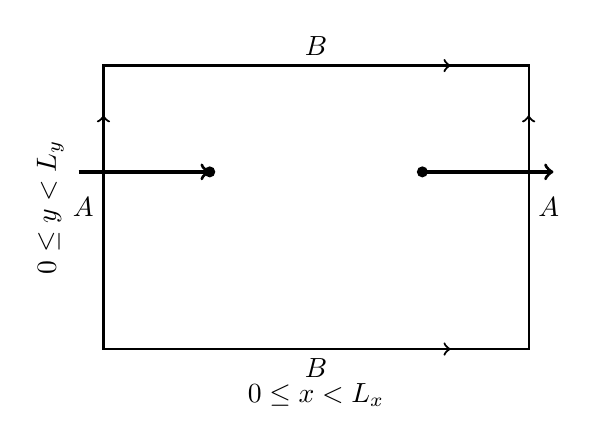
\begin{tikzpicture}[x=0.9cm,y=0.9cm]
\draw[thick] (0,0) rectangle (6,4);
\draw[->,thick] (0,0.7) -- (0,3.3);
\draw[->,thick] (6,0.7) -- (6,3.3);
\draw[->,thick] (1.1,0) -- (4.9,0);
\draw[->,thick] (1.1,4) -- (4.9,4);
\node[left] at (0,2) {$A$};
\node[right] at (6,2) {$A$};
\node[below] at (3,0) {$B$};
\node[above] at (3,4) {$B$};
\draw[->,very thick] (4.5,2.5) -- (6.35,2.5);
\draw[->,very thick] (-0.35,2.5) -- (1.5,2.5);
\fill (4.5,2.5) circle (2pt);
\fill (1.5,2.5) circle (2pt);
\node at (3,-0.65) {$0\leq x<L_x$};
\node[rotate=90] at (-0.75,2) {$0\leq y<L_y$};
\end{tikzpicture}
\caption{Espacio periódico bidimensional: se identifican los lados que llevan la misma etiqueta, de modo que una partícula que cruza un lado reaparece en el punto correspondiente del lado opuesto.}
\end{figure}

\begin{classroomqa}
\lecturetimestamp{01:50:58}
\audiencequestion{¿La construcción periódica representa el espacio o los objetos que hay en él?}
\lecturerresponse{Representa el espacio. Los objetos y los campos viven en él y obedecen sus identificaciones. Se impone la periodicidad para tratar el problema de volumen infinito; luego se elimina tomando un volumen grande y sustituyendo las sumas sobre momentos por integrales.}
\end{classroomqa}

El análogo tridimensional es un cubo con tres pares de caras opuestas identificadas. Las caras izquierda y derecha coinciden, al igual que las caras superior e inferior y las caras frontal y posterior. Una partícula que cruza cualquiera de las caras reaparece por la cara identificada con ella.\footnote{El cubo periódico y sus tres pares de caras identificadas se obtienen a partir de 01:51:27--01:52:17. La ecuación mostrada para \(k_i\) reconstruye componente a componente la condición anterior \(kL=2\pi n\), aplicada a las tres direcciones periódicas.} Las tres componentes del momento satisfacen
\begin{equation}
k_i=\frac{2\pi n_i}{L_i},
\qquad i=x,y,z,
\end{equation}
con un entero \(n_i\) para cada dirección. Se pueden definir toros en cualquier número de dimensiones siguiendo la misma regla.

\begin{figure}[t]
\centering
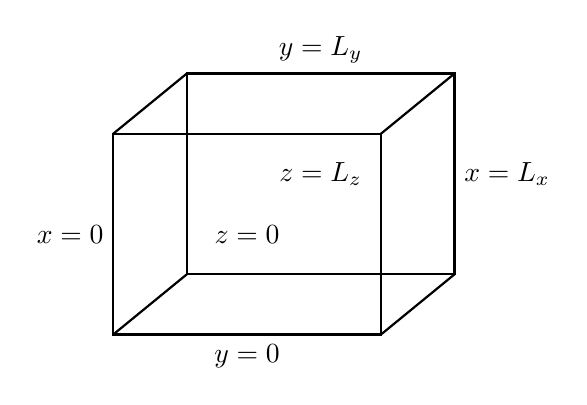
\begin{tikzpicture}[scale=0.85]
\draw[thick] (0,0) rectangle (4,3);
\draw[thick] (1.1,0.9) rectangle (5.1,3.9);
\draw[thick] (0,0) -- (1.1,0.9);
\draw[thick] (4,0) -- (5.1,0.9);
\draw[thick] (4,3) -- (5.1,3.9);
\draw[thick] (0,3) -- (1.1,3.9);
\node[left] at (0,1.5) {$x=0$};
\node[right] at (5.1,2.4) {$x=L_x$};
\node[below] at (2,0) {$y=0$};
\node[above] at (3.1,3.9) {$y=L_y$};
\node at (2,1.5) {$z=0$};
\node at (3.1,2.4) {$z=L_z$};
\end{tikzpicture}
\caption{Un espacio periódico tridimensional representado como un cubo con cada par de caras opuestas identificado.}
\end{figure}

\begin{classroomqa}
\lecturetimestamp{01:52:20}
\audiencequestion{¿La teoría de campos elige un tamaño físico para la cuadrícula espacial?}
\lecturerresponse{Es una pregunta especulativa. A efectos prácticos, aquí el espacio es continuo. Los cuantos son partículas, no celdas de una cuadrícula espacial. En la construcción del círculo, lo que se vuelve discreto es el momento; la posición sigue siendo continua y periódica.}
\end{classroomqa}

\editorialnote{Un largo pasaje dañado durante el intercambio sobre el tamaño de la cuadrícula menciona escalas de Planck, pero no conserva ninguna afirmación recuperable sobre la discreción fundamental del espacio. Aquí no se infiere tal afirmación.}

La discreción de \(k\) se debía por completo a imponer una función de onda periódica. No demuestra que la coordenada \(x\) misma forme una red. Es legítimo preguntarse si el espacio podría tener una estructura microscópica fundamental, pero se trata de una cuestión especulativa aparte.

\section{Fermiones y campos externos}

Los modos bosónicos permiten cualquier número de ocupación no negativo. Los fermiones se comportan de manera opuesta: el principio de exclusión de Pauli prohíbe que dos fermiones idénticos ocupen el mismo estado.

\begin{classroomqa}
\lecturetimestamp{01:55:13}
\audiencequestion{¿La forma más sencilla de formular una teoría de fermiones consiste en sustituir los conmutadores por anticonmutadores?}
\lecturerresponse{Sí, en esencia. El conmutador es \([A,B]=AB-BA\), mientras que el anticonmutador es \(\{A,B\}=AB+BA\). El álgebra fermiónica correspondiente de creación y aniquilación implementa la exclusión de Pauli: no se puede añadir un segundo fermión idéntico a un estado ya ocupado. El desarrollo detallado se deja para más adelante.}
\end{classroomqa}

Los dos productos se diferencian en un signo:
\begin{equation}
[A,B]=AB-BA,
\qquad
\{A,B\}=AB+BA.
\end{equation}
El conmutador es antisimétrico al intercambiar los operadores, mientras que el anticonmutador es simétrico. Si un anticonmutador se anula, entonces
\begin{equation}
\{A,B\}=0
\quad\Longrightarrow\quad
AB=-BA.
\end{equation}
Para un par así, intercambiar los dos operadores fermiónicos cambia el signo. Esto es más peculiar que la conmutación ordinaria, en la que \([A,B]=0\) implica \(AB=BA\). Sustituir los conmutadores bosónicos por el álgebra anticomutativa correspondiente es el cambio matemático que da lugar a los fermiones; su desarrollo detallado queda aplazado.

La anticonmutación invierte el comportamiento estadístico que se observa para los bosones. No hay acumulación estimulada de fermiones idénticos en un mismo modo; la ocupación de ese modo impide que entre otro fermión idéntico. Como un estado fermiónico individual puede contener como máximo un fermión idéntico, no se obtiene un límite de campo clásico introduciendo un número arbitrariamente grande de ellos en ese único estado.

\begin{classroomqa}
\lecturetimestamp{01:58:03}
\audiencequestion{¿Cómo puede ser bosón una partícula alfa si está formada por fermiones?}
\lecturerresponse{Un compuesto ligado que contiene un número par de constituyentes fermiónicos puede tener estadística bosónica. Poner varios bosones compuestos de ese tipo en el mismo estado global no equivale a poner sus constituyentes fermiónicos individuales en un mismo estado de partícula única idéntico.}
\end{classroomqa}

La estadística de un compuesto se refiere al objeto ligado en su conjunto. Por eso, los constituyentes fermiónicos pueden combinarse para formar un objeto que se comporta como un bosón sin violar la exclusión para dichos constituyentes.

\begin{classroomqa}
\lecturetimestamp{01:58:33}
\audiencequestion{¿Cómo se incorporan los campos externos?}
\lecturerresponse{Hasta ahora, la construcción no ha incluido ningún campo de fondo externo. Ese campo puede prescribirse como un campo clásico o representarse cuánticamente mediante un estado que contenga un gran número de cuantos.}
\end{classroomqa}

Para que ambas descripciones coincidan, el estado de alta ocupación debe prepararse adecuadamente y tener coherencia de fase; el número de partículas por sí solo no basta.\footnote{El intercambio introduce la escala de muchos cuantos. Aquí se especifica la coherencia de fase como condición adicional, para evitar confundir una ocupación elevada por sí sola con un campo clásico.} En ese régimen semiclásico, sus efectos concuerdan salvo por pequeñas desviaciones cuánticas. Esta es una condición básica de consistencia. El campo electromagnético debe describir fotones discretos cuando importan los cuantos individuales y, a la vez, un estado con la coherencia de fase adecuada que contenga muchos fotones debe reproducir el comportamiento conocido de una onda electromagnética clásica.
